\chapter{Homogeneous Electron Gas}

\section{Exchange and Correlation}\label{s5.1}
The homogeneous electron gas is describe by the Hamiltonian
\begin{eqnarray}
    H &=& \sum_{\bp\sigma} \varepsilon_\bp C^\dagger_{\bp\sigma} C_{\bp\sigma} + \frac{1}{2V} \sum_{\bk\bk'\sigma\sigma'} \sum_{\bq\neq 0} v_q C^\dagger_{\bk+\bq \sigma} C^\dagger_{\bk'-\bq \sigma'} C_{\bk'\sigma'} C_{\bk\sigma} \label{5.1} \\
\varepsilon_p &=& \frac{p^2}{2m} \nonumber \\
v_q &=& \frac{4\pi e^2}{q^2} \label{5.2}
\end{eqnarray}
which was derived in \eqref{1.164}.
The free electrons mutually interact by Coulomb's law.
This $N_e$ electrons in a volume $V$ with the average density $n_0 = \frac{N_e}{V}$.
A positive charge of density $n_0$ is spread uniformly through the volume make the system charge neutrality.
The homogeneous electron gas is also called the \textbf{jellium model} of a solid.

The parameter $r_s$ is universally used to describe the density of an electro gas,
\begin{equation}
    \frac{4\pi n_0 a_0^3}{3} r_s^3 =1 \label{5.3}
\end{equation}
where $a_0$ is the Bohr radius.
$r_s$ is small for high-density electron gas and it is large for a low-density gas.
The density may related to the Fermi vector,
\begin{equation}
    n_0 = 2 \int \frac{d^3 p}{(2\pi)^3} \eta_p = \frac{1}{\pi^2} \int_0^{k_F} p^2 dp = \frac{k_F^3}{3\pi^2}     \label{5.4}
\end{equation}
so the Fermi wave vector and energy are related to $r_s$,
\begin{eqnarray}
    k_F a_0 &=& \frac{1.9192}{r_s} \nonumber \\
    E_F &=& \frac{3.6832}{r_s^2}  E_{ry}, ~ ~ ~ E_{ry}=13.60 eV \label{5.5}
\end{eqnarray}
The plasma frequency is
\begin{equation}
    \hbar \omega_p = \hbar \sqrt{ \frac{4\pi e^2 n_0}{m}  }     \label{5.6}
\end{equation}
In homogeneous electron gas, the average kinetic energy of the electrons is going to be proportional to $\langle E_F \rangle \sim k_F^2$.
Which by dimension analysis, we have $\langle E_F \rangle\propto 1/r_s^2$.
For the Coulomb energy $\langle v_p \rangle \propto 1/r_s$.
When the electron gas is sufficiently hight, $r_s$ is small, the kinetic energy term will be larger than the potential energy term, which means electrons behaves like the free particles.

\subsection{Kinetic energy}
The first energy term is kinetic energy.
The contribution to the ground state energy is obtained by summing over all particles in the ground state
\begin{eqnarray}
    E &=& \sum_{\bp \sigma} \varepsilon_p n_p = 2 V \int \frac{d^3 p}{(2\pi)^3} \frac{p^2}{2m} \eta_p = \left( \frac{N_e}{n_0} \right) \frac{1}{2\pi^2 m} \int_0^{k_F} p^4 dp \nonumber \\
&=& \frac{3}{5} \frac{\hbar^2 k_F^2}{2m} N_e = \frac{3}{5} E_F N_e = \frac{2.2099}{r_s^2} E_{ry} N_e    \label{5.8}
\end{eqnarray}
The average kinetic energy is $ \frac{3}{5} E_F$, which is given in terms of $r_s$.

\subsection{Hartee}
All the remaining terms in the energy come from the Coulomb interaction between the particles.
\textit{The first term which occurs is the Coulomb interaction between the electrons and the uniform positive background}, which is called the \textbf{Hartee interaction}.
In the model of the homogeneous electron gas, the time-averaged electron density is uniform throughout the system, as is the positive background.
These equal and opposite charge cancel each other, and Hartree energy is zero.
The energy is
\begin{equation}
    N_e E_0 = \frac{e^2}{2} \int \frac{d^3 r_1 d^3 r_2}{\abs{\br_1 - \br_2}} \left[ \rho_e(\br_1) - \rho_i(\br_1) \right] \left[ \rho_e(\br_2) - \rho_i(\br_2) \right]  \label{5.9}
\end{equation}
but the ion and electron are $\rho_e = \rho_i = n_0$, then the contribution is zero.
This fact has already been used in \eqref{5.1} by omission of the $\bq=0$ term from the Coulomb interaction.
The $\bq=0$ term is the direct Coulomb interaction among the electrons, and it is omitted because it is canceled by the direct interaction with the positive background.

\subsection{Exchange}
The Coulomb interaction in \eqref{5.1} provide other energy contributions in addition to the direct term.
For Hartee term the corresponding $H$ is given
\begin{equation}
    \sum_{\bk \bk' \sigma \sigma'} \langle C^\dagger_{\bk+\bq,\sigma} C^\dagger_{\bk'-\bq,\sigma'} C_{\bk',\sigma'} C_{\bk,\sigma} \rangle \approx \delta_{\bq = 0} \sum_{\bk\sigma} \langle C^\dagger_{\bk,\sigma} C_{\bk,\sigma} \rangle \sum_{\bk'\sigma'} \langle C^\dagger_{\bk',\sigma'} C_{\bk',\sigma'} \rangle
\end{equation}
Another way to pair the same operator gives
\begin{equation}
    \approx - \sum_{\bk\bk'\sigma\sigma'} \langle C^\dagger_{\bk+\bq,\sigma} C_{\bk',\sigma'} \rangle \langle C^\dagger_{\bk'-\bq,\sigma'} C_{\bk,\sigma'} \rangle = - \sum_{\bk\sigma} n_{\bk+\bq} n_\bk
\end{equation}
This require that $\sigma' =\sigma$ and $\bk' = \bk + \bq$.
This term is called \textbf{exchange energy (Fock energy)}.
\textit{Retaining both terms is called Hartree-Fock.}
The exchange term was derived in \eqref{2.138}, it gives a contribution to the energy of an individual electron, as well as a contribution to the ground state energy of the collection of electrons. \textbf{For per electron},
\begin{equation}
    \Sigma_x(k) = - \frac{1}{V} \sum_\bq v_q n_{\bk+\bq}    \label{5.11}
\end{equation}
\begin{equation}
    E_{gx} = - \sum_{\bk\bq\sigma} \frac{v_q}{2V}   n_{\bk+\bq} n_\bk =\frac{1}{2N_e} \sum_{\bk\sigma} n_\bk \Sigma_x(k)  \label{5.12}
\end{equation}
The self-energy $\Sigma_x(k)$ depends only on the magnitude of the wave vector $k$ of the particle and gives
\begin{eqnarray}
    \Sigma_x(k) &=& - \int \frac{d^3 p}{(2\pi)^3} \frac{4\pi e^2}{\abs{\bp -\bk}^2} n_p \nonumber \\
    &=& - \frac{e^2}{\pi}  \int_0^{k_F} p^2 dp \int_{-1}^{1} \frac{d \cos\theta}{k^2+p^2 -2pk\cos\theta} \nonumber \\
    &=& - \frac{e^2 k_F}{\pi}  \left( 1+ \frac{1-y^2}{2y} \ln \abs{\frac{1+y}{1-y}}  \right) \label{5.16} \\
    y &=& \frac{k}{k_F} \label{5.17}
\end{eqnarray}

A particle at the Fermi energy $k=k_F$ has
\begin{equation}
    \Sigma_x (k_F) = - \frac{e^2 k_F}{\pi} \label{5.18}
\end{equation}
It is convenient to write
\begin{eqnarray}
    \Sigma_x(k) &=& \frac{e^2 k_F}{\pi} S(y)    \label{5.19} \\
    S(y) &=& - \left( 1+ \frac{1-y^2}{2y} \ln \abs{ \frac{1+y}{1-y} } \right)   \label{5.20}
\end{eqnarray}
where $S(y)$ is a function which gives the wave vector dependence of the exchange energy.
\begin{figure}[ht]
    \centering
    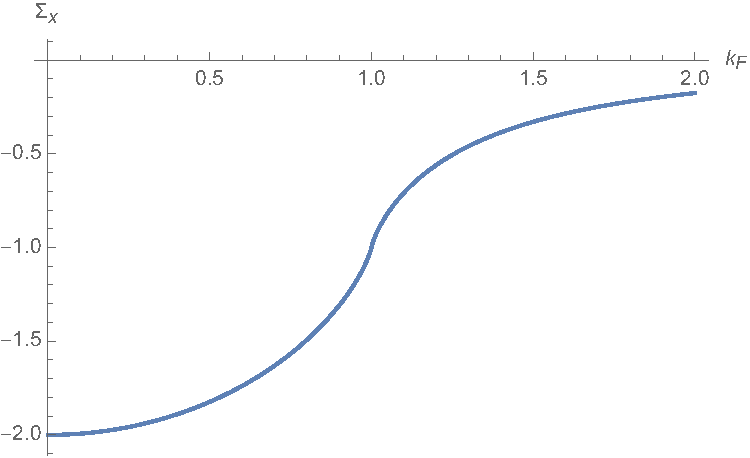
\includegraphics[width=0.4\linewidth]{./fig/fig5_1.pdf}
    \caption{Exchange energy.}%
    \label{fig:5.1}
\end{figure}
The behaviour of the function is in shown in Figure~\ref{fig:5.1}.

The derivative has a logarithmic divergence as $y\to 1$. This fact is interesting because it predicts that the effective mass is zero.
The effective mass of a particle defined in \eqref{3.160}.
Since the exchange self-energy is not frequency dependent, the effective mass is
\begin{equation}
    \left( \frac{m}{m^*} \right) = 1+ \partial_{\varepsilon_k} \Sigma_x(k) = \frac{e^2 m}{2\pi k_F } \frac{1}{y^2} \left( \frac{1+y^2}{y} \ln \abs{ \frac{1+y}{1-y} }-1  \right) \label{5.24}
\end{equation}
which diverges at Fermi energy $y\to 1$.
If the inverse effective mass really diverged at the Fermi surface, it would have several observable consequences.
The electron gas would be unstable at low temperatures, and the specific heat would diverge.
Further terms in the perturbation theory produces another divergence in the effective mass which exactly cancels the one due to exchange.
The effective mass and specific heat are not divergent.

The exchange energy contribution to the ground state energy is obtained from \eqref{5.12}.
Summing over spin gives an expression
\begin{eqnarray}
    E_{gx} &=& \frac{1}{N_e} \sum_\bk n_\bk \Sigma_x(k) = \frac{1}{n_0} \int \frac{d^3k}{(2\pi)^3} n_k \Sigma_x(k) \nonumber \\
    &=& - \frac{3}{4} \frac{e^2 k_F}{\pi} \label{5.25}
\end{eqnarray}
The average exchange energy per electron is $ \frac{3}{2} $ of the value ate the Fermi energy.
In therms of the parameter $r_s$, the total ground state exchange energy per electron is
\begin{equation}
    E_{gx} = - \frac{3}{2\pi} (k_F a_0) \left( \frac{e^2}{2a_0} \right) = - \frac{0.9163}{r_s} \label{5.26}
\end{equation}

So far two terms have been found for the energy of the particle,
\begin{equation}
    E(k) = \frac{\hbar^2 k^2}{2m} + \Sigma_x(k) + \dots \label{5.27}
\end{equation}
The corresponding two terms for the ground state energy per particle are,
\begin{equation}
    E_g = \frac{2.2099}{r_s^2} - \frac{0.9163}{r_s} + \dots \label{5.28}
\end{equation}
The ground state energy has the appearance of a power series, in increasing powers of $r_s$.
Although it is usually unsafe to extrapolate from just two terms, in fact $E_g$ is a series in $r_s$.
The next term will be of order $O(r_s^0)$.
The zeroth power could be interpreted as either a constant or as $\ln(r_s)$.
The series have the form
\begin{equation}
    E_g =  \frac{2.2099}{r_s^2} - \frac{0.9163}{r_s} -0.094 + 0.0622\ln(r_s) + \dots \label{5.29}
\end{equation}

The above energy terms comprise the Hartree-Fock theory.
It is defined to be the kinetic energy, the Hartree energy which is zero, and the exchange energy.
The total ground state energy per particle is written with correlation energy,
\begin{equation}
    E_g = \frac{2.2099}{r_s^2} - \frac{0.9163}{r_s} +E_c \label{5.30}
\end{equation}
where the correlation energy $E_c$ needs to be determined.
The result
\begin{equation}
    E_c = -0.094 + 0.0622\ln(r_s) + O(r_s) \label{5.31}
\end{equation}
is convergence when $r_s \leq 1$.

\subsection{Seitz's Theorem}
The theorem of Seitz relates the ground state energy to the chemical potential.
The chemical potential is defined as the energy it takes to add or remove an electron from the material.
It is the energy which divides the empty from the occupied states at zero temperature.
Of course, it is just the Fermi energy of the metal.
The chemical potential is the energy of an electron of momentum $k_F$
\begin{equation}
    \mu = \frac{\hbar^2 k_F^2}{2m} + \Sigma_x (k_F) + \Re \Sigma_c(k_f,0) \label{5.33}
\end{equation}
where $ik_n= 0$ is the chemical potential.
The chemical potential $\mu$ is only a function of the electron $n_0$. The theorem of Seitz is
\begin{equation}
    \mu (n_0)  = \frac{d}{d n_0}  \left[ n_0 E_g(n_0) \right] = E_g + n_0 \frac{d E_g}{d n_0} \label{5.34}
\end{equation}
The proof, by definition of chemical potential
\begin{equation}
    \mu = E_T(N_e+1) - E_T(N_e)     \label{5.35}
\end{equation}
The total energy for $N_e$ particle system is $E_T = N_e E_g$ for a fixed volume since the $E_g$ is the function of density,
\begin{eqnarray}
    E_T(N_e+1) &=& (N_e+1) E_g(n_0 + 1/V) = (N_e+1) \left( E_g(n_0) + \frac{1}{V} \frac{d E_g}{d n_0} \right) \nonumber \\
    &=& N_e E_g + E_g(n_0) + n_0 \frac{dE_g}{n_0}  + O( \frac{1}{V} )   \label{5.36}
\end{eqnarray}
In proving the theorem, the volume $V$ is kept fixed, as is the amount of positive charge.
The $N_e+1$ particle system has a slight charge imbalance, but it is negligible to the contribution of energy.
Considering a body of average dimension $L$ is uniformly charged with on unit of charge, the Coulomb energy is of order $e^2/L$.
This contribution is negligible when $L$ is large.

The chemical potential is the negative of the work function.
It is the energy required to remove an electron form the solid and take it to infinity with zero kinetic energy.
However, there is a surface correction to the work function, but not to volume part of the ground state energy per particle.
\begin{equation}
    E_T = N_e E_g + A E_S   \label{5.37}
\end{equation}
where $A$ is the total surface area and $E_S$ is the energy per unit surface area.
For macroscopic bodies, $E_g$ does not depend on the surface area.
However, $\mu$ does have a term which depends on the surface--actually on the surface dipole layer, $\mu = \mu_B + \Delta \mu$.
The theorem of Seitz actually just works on $\mu_B$.
In Hartree-Fock approximation the chemical potential gives for the bulk contribution,
\begin{equation}
    \mu_{B,HF} = \frac{d}{dn_0} \left( n_0 E_{g,HF} \right) = E_F - \frac{e^2 k_F}{\pi}     \label{5.39}
\end{equation}

\subsection{$\Sigma^{2a}$}
The exchange energy calculated involve one Coulomb line.
The correlation energy is the sum of all contribution with two or more Coulomb lines.
There are three diagrams with two Coulomb line.
\begin{figure}[ht]
    \centering
    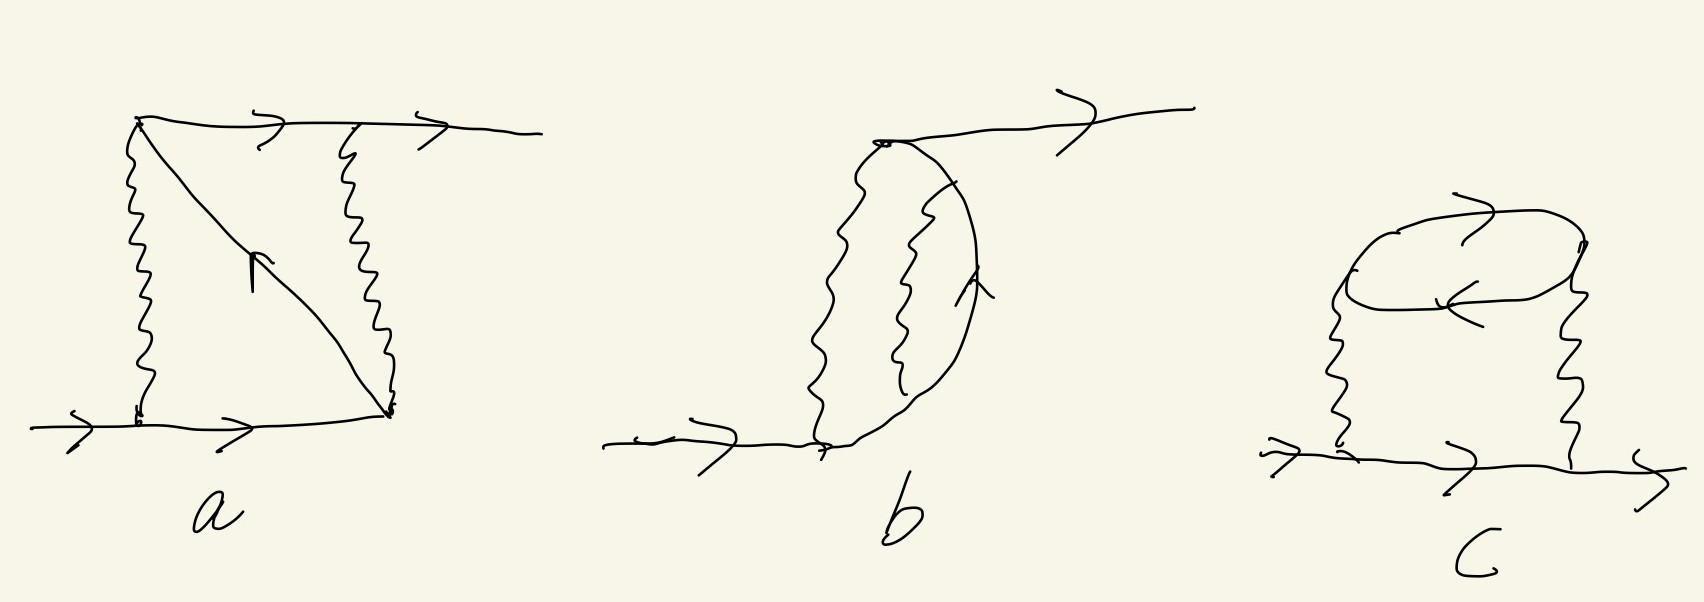
\includegraphics[width=0.8\linewidth]{./fig/fig5-2.jpg}
    \caption{Diagrame}%
    \label{fig:5.2}
\end{figure}

For Figure~\ref{fig:5.2}a, the self-energy contribution is
\begin{equation}
    \Sigma^{2a}(k) = \frac{1}{V^2\beta^2} \sum_{\bq \bq'} v_q v_{q'} \sum_{iq_n,iq_{ n'}} \cg^0(k+q) \cg^0(k+q') \cg^0(k+q+q')
\end{equation}
according \eqref{3.217} and calculation, we have
\begin{eqnarray}
    \Sigma^{2a}(k) &=& - \frac{1}{V^2} \sum_{\bq \bq'} \frac{v_q v_{q'}}{ik_n + \xi_{\bk+\bq+\bq'} - \xi_{\bk+\bq'} -\xi_{\bk+\bq} } \nonumber \\
    &=& \left[ \eta_F(\xi_{\bk+\bq'}) \left( \eta_F(\xi_{\bk+\bq}) - \eta_F(\xi_{\bk+\bq+\bq'})  \right) \right. \nonumber\\
    &+&\left. \eta_F(\xi_{\bk+\bq+\bq'})\left( 1- \eta_F(\xi_{\bk+\bq} \right) \right]
\end{eqnarray}
The self-energy of a particle is needed on the Fermi surface.
Set $k=k_F$ and $ik_n = \xi_{k_F} =k_F^2/2m - \mu = 0$.
The terms in the energy denominator largely cancel,
\begin{equation}
    \xi_\bk + \xi_{\bk+\bq+\bq'} - \xi_{\bk+\bq} - \xi_{\bk+ \bq'} = \frac{\bq \cdot \bq'}{m}   \label{5.44}
\end{equation}
The self-energy is
\begin{eqnarray}
    \Sigma^{2a}(k_F,0) &=& - \frac{(4\pi e^2)^2 m}{(2\pi)^6} \int \frac{d^3 q}{q^2} \int \frac{d^3 q'}{(q')^2} \frac{1}{\bq \cdot \bq'} \nonumber \\
    &\times& \{ \eta_F(\xi_{\bk+\bq'}) \left[ \eta_F(\xi_{\bk+\bq}) - \eta_F(\xi_{\bk+\bq+\bq'})  \right] + \dots  \} \label{5.45}
\end{eqnarray}
The quantity on the right is independent of the electron density.
The integral is convergent and give nonzero result.
It contribute the constant term in $E_c$.
With further calculation by Onsager, we have
\begin{equation}
    \Sigma^{2a} = \frac{1}{3} \ln(2) - \frac{3}{2\pi^2}  \zeta(3) = 0.0436
\end{equation}

\subsection{$\Sigma^{2b}$}
The second self-energy term involving two Coulomb lines is shown in Figure~\ref{fig:5.2}b, this contribution can be shown equal to zero.
Consider the summation of the similar diagrams, all terms may be summed by evaluating the exchange energy with an electron Green's function in the self-energy which includes the exchange energy.
This summation is given by the self-energy
\begin{equation}
    \Sigma'_x(k) = - \frac{1}{V\beta} \sum_{\bq,ik_n} v_q \cg(\bk+\bq,ik_n) \label{5.47}
\end{equation}
\begin{equation}
    \cg (\bk+\bq,ik_n) = \frac{1}{ik_n - \xi_{\bk+\bq} -\Sigma_x(\bk+\bq)} \label{5.48}
\end{equation}
where the Green's function has a self-energy due to exchange.
Since the self-energy $\Sigma_x(k)$ does not depend on frequency, the frequency summation of the Green's function yields the simple number operator as in \eqref{3.219}
\begin{equation}
    \frac{1}{\beta}  \sum_{ik_n} \cg \left(\bk + \bq, ik_n\right) = \eta_F\left[ \xi_{\bk+\bq} + \Sigma_x(\bk+\bq)  \right] = \frac{1}{e^{\beta(\xi+\Sigma)}+1}
\end{equation}
and the self-energy of \eqref{5.47} is
\begin{equation}
    \Sigma'_x (k) = - \frac{1}{V} \sum_\bp v_{\bp-\bk} \eta_F \left[ \xi_\bp + \Sigma_x(\bp)  \right]  \label{5.49}
\end{equation}
At zero temperature the electron distribution function is a step function.
\textbf{This step function must also be normalized so that the electron density is still $n_0$}, as
\begin{equation}
    n_0 = 2 \int \frac{d^3 p}{(2\pi)^3} \eta_F \left[ \xi_p + \Sigma_x(p) \right]   \label{5.50}
\end{equation}
The effect of the exchange energy $\Sigma_x(p)$ in the argument of $\eta_F$ is to change the chemical potential.
\textbf{However, the Fermi wave vector $k_F$ is the same, even after the exchange energy has been included in the occupation function}.
Since the Fermi wave vector determines by the density $n_0$.
Thus the addition of the exchange energy must be canceled by an equal change in chemical potential, at zero temperature
\begin{equation}
    \lim_{T\to 0} \eta_F\left[ \xi_k + \Sigma_x (k) \right] = \Theta ( k_F - k)   \label{5.51}
\end{equation}
The exchange energy $\Sigma'_x(k)$ in \eqref{5.49} is exactly equal to the one calculated earlier.
Thus the summation of all terms just yields the value of the first term alone.
All of the subsequent terms in that series sum to zero, because of a shift in the chemical potential.

The exchange self-energy has a remarkable effect upon the zero temperature electron distribution.
It leaves $k_F$ unchanged. This simple result is a consequence of the feature that $\Sigma_x(k)$ is independent of frequency.

\subsection{$\Sigma^{2c}$}
The third self-energy with two Coulomb lines is written as
\begin{equation}
    \Sigma^{2c}(k) = - \frac{1}{V\beta}  \sum_{\bq,iq_m} v_q^2 \mathcal{P}^{(1)}(\bq,iq_m) \cg^0 (\bk+ \bq,ik_n+iq_m)   \label{5.52}
\end{equation}
The closed fermion loop gives the polarization diagram $\mathcal{P}^{(1)}(\bq,iq_m)$ \footnote{Eq.3.214 in the book}.
This diagram has one drawback.
The wave vector integral appears to diverge at small values of $q$, because of the factor $v_q^2$,
\begin{equation}
    \int \frac{d^3 q}{q^4} \Longrightarrow \int_0 \frac{dq}{q^2} \to \infty \label{5.53}
\end{equation}
So this self-energy term is infinite.
The divergence is removed by summing a series of self-energy diagram, as shown Fig.~\ref{fig:5.3}.
\begin{figure}[ht]
    \centering
    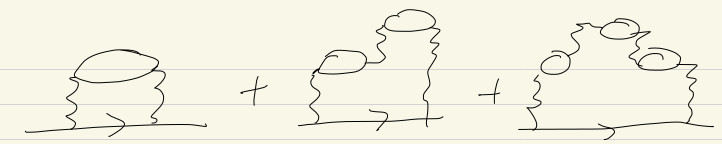
\includegraphics[width=0.8\linewidth]{fig/fig5-3.jpg}
    \caption{Summation of diagram.}%
    \label{fig:5.3}
\end{figure}
Each term has one more polarization bubble and one more Coulomb line--hence an additional factor of $v_q\mathcal{P}^{(1)}$.
The summation of these terms gives the simple series
\begin{eqnarray}
    \Sigma^{c}(k) &=& - \frac{1}{V\beta}  \sum_q v_q \cg^{(0)} (k+q) \nonumber \\
    &\times& \lbrace v_q \mathcal{P}^{(1)}(q) + \left[ v_q \mathcal{P}^{(1)}(q) \right]^2 + \left[ v_q \mathcal{P}^{(1)}(q) \right]^3 + \dots \rbrace \nonumber \\
    &=& - \frac{1}{V\beta} \sum_q v_q \cg^{(0)}(k+q) \frac{v_q \mathcal{P}^{(1)}(q)}{1 - v_q \mathcal{P}^{(1)}(q)} \label{5.54}
\end{eqnarray}
The summation of terms shown in Fig.~\ref{fig:5.3} is called the \textbf{random phase approximation (RPA)}.
The approximation in RPA is that this series of terms is used to represent the entire answer.
RPA ignores other terms, such as \eqref{5.45}, which was found from the diagram in Fig.~\ref{fig:5.2}(a).
RPA ignores many more terms in each higher order of perturbation series.

The denominator in \eqref{5.54} is a very important quantity because it is very often used in calculations.
It is the RPA approximation to the dielectric function and is defined as
\begin{equation}
    \varepsilon_{RPA} (q) = 1 - v_q \mathcal{P}^{(1)}(q)    \label{5.55}
\end{equation}
Then the self-energy series may be written as
\begin{equation}
    \Sigma^c(k) = - \frac{1}{V\beta}  \sum_q v_q \cg^{(0)}(k+q) \left[ \frac{1}{\varepsilon_{RPA}(q)}-1  \right]    \label{5.56}
\end{equation}
Remember the exchange energy term in \eqref{5.47}, which is exactly the $-1$ term.
Then adding the exchange energy to the above result gives a term containning the $RPA$ dielectric function
\begin{equation}
    \Sigma_{RPA}(k) = \Sigma^c(k) + \Sigma_x(k) = - \frac{1}{V\beta}  \sum_q v_q \frac{\cg^{(0)}(k+q)}{\varepsilon_{RPA}(q)} \label{5.58}
\end{equation}
The summation of these two terms is define as the \textbf{RPA self-energy} or called \textbf{screened exchange energy}.
With this correction, the inverse effective mass no longer diverges at the Fermi surface as will shown later.

\subsection{Hight=Density Limit}
In RPA the correlation energy is
\begin{equation}
    E_{c,RPA} = -0.142 + 0.0622 \ln r_s + O(r_s, r_s \ln(r_s))  \label{5.59}
\end{equation}
Adding the Onsager result, for the second-order diagram $\Sigma^{(2a)}$ in \eqref{5.45}, gives the result of Gell-Mann and Bruckner
\begin{equation}
    E_c = -0.094 + 0.0622 \ln r_s + \dots   \label{5.60}
\end{equation}
Another term is obtained by Carr and Maradudin
\begin{equation}
    E_c = -0.094 + 0.0622 \ln r_s + 0.018 r_s \ln r_s + a r_s + O(r_s^2)   \label{5.61}
\end{equation}
In high density limit, $r_s \to 0 $, the energy in \eqref{5.61} is not analytic, but the series is accurate in this limit.
For metallic the density is around $1.8<r_s<56$, in this region  the perturbation formula for $E_c$ is not valid, because the correlation energy must be negative.

\subsection{Pair Distribution Function}
The correlation energy is the improvement in the ground state energy beyond the Hartree-Fock approximation.
It is useful to examine an important property of the Hartree-Fock theory, the pair distribution function $g(r)$, to understand the correlation energy.
The pair distribution function $g(r)$ is the probability per unit volume that an election is at $\br$ is there is already one at $\br=0$.
There are two different pair distribution functions in an unmagnetized electron gas: $g_{\uparrow\uparrow}(\br) = g_{\downarrow\downarrow}(\br)$ and $g_{\uparrow\downarrow}(\br) = g_{\downarrow\uparrow}(\br)$ \footnote{The first is the spin for $\br=0$.}.
Of course, the electrons are not fixed, and they are usually moving rapidly.
Then these pair distribution functions are averages for the moving particles.
Even the electron at $\br=0$ is not fixed, so that this reference point moves with the electron.

The N-particle wave function is a Slater determinant,
\begin{equation}
    \Psi_{\lambda_1,\lambda_2,\dots \lambda_N}(\br_1 \dots \br_N) = \frac{1}{\sqrt{N!}}
    \begin{bmatrix}
        \phi_{\lambda_1}(\br_1) & \phi_{\lambda_1}(\br_2) & \dots & \phi_{\lambda_1}(\br_N) \\
        \phi_{\lambda_2}(\br_1) & \phi_{\lambda_2}(\br_2) & \dots & \phi_{\lambda_2}(\br_N) \\
        \vdots & \vdots & \ddots & \vdots \\
        \phi_{\lambda_N}(\br_1) & \phi_{\lambda_N}(\br_2) & \dots & \phi_{\lambda_N}(\br_N)
    \end{bmatrix} \label{5.62}
\end{equation}
where the $\lambda_j$ are the quantum numbers which describe the states, and there is one wave function for every occupied electron state.
The pair distribution function is given by the two-particle density matrix, by integrating the N-particle density wave function
\begin{equation}
    g_{ss'}(\br_1,\br_2) = V^2 \int d\br_3 d\br_4 \dots d \br_N \abs{\Psi_{\lambda_1 \lambda_2 \dots \lambda_N}(\br_1 \dots \br_N) }^2 \label{5.63}
\end{equation}
If the one-electron orbital $\phi_{\lambda_j}(\br)$ are assumed orthogonal, then this integration just yield the sum over all possible pair wave function,
\begin{equation}
    g_{ss'}(\br_1 ,\br_2) = \frac{V^2}{N(N-1)} \sum_{\lambda_i,\lambda_j}
    \begin{bmatrix}
        \phi_{\lambda_i}(\br_1) & \phi_{\lambda_i}(\br_2) \\
        \phi_{\lambda_j}(\br_1) & \phi_{\lambda_j}(\br_2)
    \end{bmatrix}^2
    \label{5.64}
\end{equation}
The sum over $\lambda_i$, $\lambda_j$ is over all occupied state, so each pair is summed twice.
For the homogeneous electron gas, the orbitals must describe plane wave,
\begin{equation}
    \phi_\lambda(\br) = \frac{\chi_s}{\sqrt{V}} e^{i\bk\cdot\br}    \label{5.65}
\end{equation}
where the $\chi_s$ are the sin functions.
Due to the orthogonal and normalize condition, the spin averages are $\langle \chi_\uparrow \chi_\uparrow \rangle =1$, $\langle \chi_\uparrow \chi_\downarrow \rangle =0$.
The two pair distribution functions are
\begin{eqnarray}
    g_{\uparrow\downarrow}(\br_1-\br_2) &=& \frac{1}{N(N-1)}   \sum_{\bk_1 \bk_2} \left( \abs{e^{i\bk_1\cdot \br_1 + i \bk_2 \cdot \br_2}}^2 + \abs{e^{i \bk_1\cdot \br_2 + i \bk_2 \cdot \br_1}}^2  \right) \nonumber \\
    &=& \frac{2}{N(N-1)} \left( \frac{N}{2} \right)^2 = \frac{1}{2}  \label{5.66} \\
    g_{\uparrow\uparrow}(\br_1-\br_2) &=& \frac{1}{N(N-1)}  \sum_{\bk_1 \bk_2} \abs{e^{i\bk_1\cdot\br_1 +i\bk_2\cdot\br_2} - e^{i\bk_1\cdot\br_2+ i \bk_2\cdot \br_1}}^2    \nonumber \\
    &=& \frac{1}{2} \left[ 1 - \Lambda(\br_1 -\br_2)^2 \right]  \label{5.67} \\
    \Lambda(\br) &=& \frac{2}{N} \sum_\bk e^{i\bk\cdot\br}  \label{5.68}
\end{eqnarray}
The summation over $\bk$ runs only over occupied states.
The antiparallel spin distribution function $g_{\uparrow\downarrow}=g_{\downarrow\uparrow}= 1/2$ in the Hartree-Fock approximation.
The cross term which results from the determinant is zero because of the orthogonality of the two spin functions.
There is no correlation in the position of electrons of opposite spin.
The parallel spin $g_{\uparrow\uparrow}=g_{\downarrow\downarrow}$ has a definite spatial dependence, which comes from the cross term which is retained since the spins are parallel and the spin averages are unity.
The function $\Lambda(\br)$ is calculated
\begin{equation}
    \Lambda(\br) = \frac{2}{n_0} \int \frac{d^3 k}{(2\pi)^3} \eta_k e^{i\bk\cdot\br} = \frac{3}{rk_F^3} \int_0^{k_F} kdk \sin(kr) = \frac{3}{rk_F} j_1(rk_F)    \label{5.69}
\end{equation}
where $j_1(x)$ is spherical Bessel function.
This gives the parallel spin $g_{\uparrow\uparrow}(r)$ vanish as $r=0$ and approaches $\frac{1}{2}$ at large distance.

The total pair distribution function for a particle is the combination of the result for parallel and antiparallel spin distributions,
\begin{equation}
    g(r) = g_{\uparrow\uparrow}(r) + g_{\uparrow\downarrow}(r)  \label{5.70}
\end{equation}
In a nonmagnetic system, the same result is obtained if the central particle has spin down.

The pair distribution function has two features which are important for later discussion.
First, there is the normalization integral,
\begin{equation}
    n_0 \int d\br \left[ g(\br) -1 \right] =-1  \label{5.71}
\end{equation}
The second is a statement about the ground state energy of the electron gas.
It has kinetic energy plus Coulomb parts.
The Coulomb energy around the hole in the Hartree-Fock approximation is
\begin{equation}
    E_{Coul} = \frac{e^2 n_0}{2} \int d \br \frac{g(\br)-1}{\br}    \label{5.72}
\end{equation}
The integral $E_{Coul}$ is related to the exchange energy which is discussed later in \ref{s5.6}.
The above two relations for $g(\br)$ can be checked in the Hartree-Fock approximation.
In the case of $g(\br)=1/2 + g_{\uparrow\uparrow}(\br)$, the normalization integral yields ($x=rk_F$).
\begin{equation}
    n_0 \int d \br \left[ g_{\uparrow\uparrow}(\br) - \frac{1}{2} \right] = - \frac{n_0}{2} \int d^3 r \Lambda(r)^2 = -\frac{6}{\pi} \int_0^\infty dx j_1(x)^2 = -1     \nonumber
\end{equation}
and the Coulomb integral yields
\begin{equation}
    E_{Coul} = - \frac{3 e^2 k_F}{4\pi}     \label{5.73}
\end{equation}
These result are correct for Hartree-Fock. It is the same exchange energy per particle which was derived by diagrammatic means.

The pair distribution function $g(\br)$ is the distribution of electrons, on the average, about any electron.
It goes to unity at large distance, which is a result of the uniform distribution $n_0$ of electron charge.
That is, the electron charge density is $-en_0g(\br)$.
Since $g(\br)$ is less than unity near $\br \to 0$, the electron charge is depleted in the vicinity of electron.
This reduction may be viewed as a hole in the electron density.
Wigner suggested the name \textbf{exchange and correlation hole}.
The hole moves with the electron.

According to the normalization \eqref{5.71}, the total charge missing from this hole is one electron charge.
The factor $-n_0(g-1)$ is the density of hole charge, which integrates to $1$.
The homogeneous electron gas has a uniform charge density only on the average.
To a particular electron, the system is not uniform at all, since other electrons are not as likely to venture near to it as they are to other points.

The Coulomb integral \eqref{5.73} gives the potential energy of the system.
The electron interacts with its own hole charge.
It is not influenced by the electrons or uniform charge density farther away,since they cancel on the average.
Near the electron the positive background charge is not canceled by the other electrons, since the other electrons are not as likely to be nearby.
In the Hartree-Fock approximation, only electrons of parallel spin make the exchange and correlation hole.
Since $g_{\uparrow\downarrow}=1/2$, the antiparallel spin are not affected.

It is possible to arrange $g(r)$ so that the sum rule \eqref{5.71} is still obeyed, yet the potential energy is lower than found in Hartree-Fock.
This lowering is done by permitting $g_{\uparrow\downarrow}=1/2$ to become less than $1/2$ near the point $\br \to 0$.
It is these charges which give rise to the correlation energy.
Charges in $g_{\uparrow\downarrow}$ and $g_{\uparrow\uparrow}$ will usually cost some kinetic energy, so that one cannot just adjust $g_{ss'}$ to maximize the potential energy alone.
The system will seek the lowest energy stat at $T=0$, which is the state with some "correlation" between the motion of electrons  with antiparallel spins.
This "correlation" between the motion of pairs of electrons is what gives rise to the "correlation energy".

\section{Wigner Lattice}\label{s5.2}
Actual electron systems exist over a range of densities.
For metals usually we have $1.8<r_s<6$.
The correlation energy in the high density limit, $r_s\to 0$, have been discussed in previous section.
For low-density limit and final formulas for intermediate rages was given by Wigner
\begin{equation}
    E_c = \frac{0.88}{r_s + 7.8} E_{ry} \label{5.74}
\end{equation}
and still widely used.
At low densities, Wigner speculated that the electrons would become localized and form a regular lattice.
With the jellium model where the positive charge is uniformly spread through the system.
The electron lattice would presumably be a close-packed structure such as bcc, fcc or hcp, in which electrons would vibrate around their equilibrium positions.
The localization cannot occur until the zero point energy is less than the potential energy.

Consider the Wigner-Seitz model for the unit cell of the lattice.
With a sphere of radius $r_s a_0$ a electron locate at the center.
\textit{Each sphere has overall neutrality, since the one-electron charge at the center is canceled by the positive charge inside the volume of the sphere}.
Outside of each sphere, the electric field is zero.
If all unit cells are neutral spheres, then they exert no electric fields on each other.
The electric fields inside a sphere arise only from the electron and positive charge within that sphere.
This approximation made by Wigner-Seitz assumption is remarkably small.

The first term is the potential energy between the electron and the \textit{uniform} positive background. This give
\begin{eqnarray}
    E_{ep} &=& \int d^3 \left(- \frac{e^2}{r} \right) n_0 = - \frac{3 e^2}{r_s^3 a_0^3} \int_0^{r_s a_0} r dr \nonumber \\
    &=& - \frac{3e^2}{2 a_0 r_s} = - \frac{3}{r_s} \left( \frac{e^2}{2 a_0} \right)  \label{5.75}
\end{eqnarray}
where $-e^2/r$ is the potential energy and $n_0= 3/(4\pi r_s^3 a_0^3)$ is the density of positive charge at each distance $r$.

The second term in the potential energy is the interaction of the positive charge with itself.
The potential energy $V(r)$ from the positive charge at a distance $r$ form the center is obtained by solving first for its equivalent electric field,
\begin{equation}
    - \frac{dV}{dr} =  eE(r) = \frac{e^2}{r^2} n_0 \left( \frac{4 \pi r^3}{3} \right) = \frac{e^2 r}{r_s^3 a_0^3} \label{5.76}
\end{equation}
which is $e^2/r^2$ times the total charge within the sphere of radius $r$.
Integrating this equation to obtain $V(r)$, there is a constant of integration.
It is determined by the condition that the total potential, from electron and positive charge, must vanish at the surface of the sphere.
The constant is chosen to make $V(r)$ be $e^2/r_s a_0$ at the surface.
The result is
\begin{equation}
    V(r) = \frac{e^2}{2 r_s a_0 } \left[ 3 - \left( \frac{r}{r_s a_0} \right)^2  \right] = \frac{1}{r_s} \left[ 3 - \left( \frac{r}{r_s a_0} \right)^2 \right] E_{ry}   \label{5.77}
\end{equation}
The potential energy of the positive charge interacting with itself is found using
\begin{eqnarray}
    E_{pp} &=& \frac{1}{2} \int d^3 r V(r) n_0 = \frac{3}{4}  \frac{e^2}{(r_s a_0)^4} \int_0^{r_s a_0} r^2 dr \left[3 - \left( \frac{r}{r_s a_0} \right)^2 \right] \nonumber \\
    &=& \frac{3}{5} \frac{e^2}{r_s a_0} = \frac{6}{5 r_s}  E_{ry} \label{5.78}
\end{eqnarray}
The result is multiplied by $1/2$ because it is a self-energy.
There are only two potential energy terms.
The interaction of the electron with itself is not included.
Aside form the fact that it is infinity, it does not change the metal and so does not contribute to the cohesive energy of the system.

The sum of these two terms is the total potential energy in the Wigner lattice in the Wigner-Seitz approximation.
It is a large term , it has a larger coefficient than the exchange and correlation energies which is found for the free-particle system.
The system apparently has gained energy by the localization of the electrons.

The Wigner lattice is stable in the large value of $r_s$.

\section{Metallic Hydrogen}\label{s5.3}
Skip

\section{Linear Screening}\label{s5.4}
Screening is one of the most important concepts in many-body theory.
Charges, which are able, will move in response to an electric field.
This charge movement will stabilize into a new distribution of charge around the electric field and this new distribution is just the right amount of charge to cancel the electric field at large distance.
If the electric field is caused by an impurity charge distribution $\rho_i$ with net charge $Q_i$, the amount of mobile charge attached to the surrounding is exactly $-Q_i$.
The name screening charge is applied to the mobile charge attached by the impurity electric field with own distribution in space $\rho_s$.
The screened potential from the impurity charge and the screening charge is given by
\begin{equation}
    \phi(\br) = \int d\br' \frac{\rho_i(\br') + \rho_s(\br')}{\abs{\br-\br'}}    \label{5.89}
\end{equation}

The screening charge is not necessarily in bound states due to the electric field from the impurity\footnote{That could happen if the electric field from the impurity is strong enough.}.
But quite often the screening charge is from the unbound conduction electrons of the metal or semiconductor.
In their motion through the crystal, they spend a little more time near the impurity potential, if it is attractive, than they do elsewhere in the solid.
When this motions are averaged, there is more electron density near the impurity than elsewhere, which is the screening charge.
For repulsive interaction the screening charge is similar but with positive charge since it reduce the average density of electrons.

The classical macroscopic theory give the electric field and displacement as
\begin{eqnarray}
    \nabla \cdot \mathbf{D}(\br) &=& 4\pi \rho_i(\br) \label{5.90} \\
    \nabla \cdot \mathbf{E}(\br) &=& 4\pi [ \rho_i(\br) + \rho_s(\br)] \label{5.91}
\end{eqnarray}
with Fourier-transformation
\begin{eqnarray}
    i\bq \cdot \mathbf{D}(\bq) &=& 4 \pi \rho_i(\bq) \label{5.92} \\
    i\bq \cdot \mathbf{E}(\bq) &=& 4 \pi [ \rho_i(\bq) + \rho_s(\bq) ] \label{5.93}
\end{eqnarray}
For the components that along the direction $\bq$ are the longitudinal fields $D_l$ and $E_l$.
The longitudinal electric field is related to the scalar potential,
\begin{eqnarray}
    E_l(\br) &=& - \nabla \phi(\br) \\
    \phi(\bq) &=& i \frac{E_l(\bq)}{q}
\end{eqnarray}
These gives us the result
\begin{eqnarray}
    D_l(\bq) &=& \frac{4\pi}{iq} \rho_i(\bq)    \label{5.94} \\
    E_l(\bq) &=& \frac{4\pi}{iq} [\rho_i(\bq) + \rho_s(\bq)] \label{5.95} \\
    \phi(\bq) &=& \frac{4\pi}{q^2} [ \rho_i(\bq) + \rho_s(\bq)] \label{5.96}
\end{eqnarray}
The \textbf{dielectric response function} is defined as the ration of $ \frac{D_l(\bq)}{E_l(\bq)} $ int he limit where $\rho_i \to 0$
\begin{equation}
    \varepsilon(\bq) = \lim_{\rho_i \to 0} \frac{D_l(\bq)}{E_l(\bq)} = \lim_{\rho_i \to 0} \left[ \frac{\rho_i(\bq)}{\rho_i(\bq)+ \rho_s(\bq)} \right]  \label{5.97}
\end{equation}
In this limit $\varepsilon(\bq)$ becomes a property of the material and is independent of the charge distribution.

To calculate the dielectric function.
The linear screening model assumes this definition of \eqref{5.97} is true for nonzero $\rho_i(\bq)$, which gives for the potential
\begin{eqnarray}
    \phi'(\bq) &=& \frac{4\pi}{q^2} \frac{\rho_i(\bq)}{\varepsilon(\bq)} \label{5.98} \\
    \phi'(\br) &=& \int \frac{d^3 q}{(2\pi)^3} \frac{4\pi}{q^2} \frac{\rho_i(\bq)}{\varepsilon(\bq)} e^{i\bq\cdot\br} \label{5.99}
\end{eqnarray}
The potential $\phi'$ is the total potential from screening charge and impurity charge.
The potential $\phi'$ should be similar to the exact screened potential $\phi$ in \eqref{5.89} and they are identical in the limit where $\rho_i$ is small.
The linear screening approximation is to calculate $\phi'$ in place of $\phi$.
Another feature of the linear screening model is that the screening charge $\rho_s(\bq)$ density is proportional, in $\bq$ space, to the impurity charge density $\rho_i(\bq)$.
Linear screening model assume that
\begin{eqnarray}
    \varepsilon (\bq) &=& \frac{\rho_i(\bq)}{\rho_i(\bq) + \rho_s(\bq)} \label{5.100} \\
    \frac{\rho_s(\bq)}{\rho_i(\bq)} &=& \frac{1}{\varepsilon(\bq)} -1   \label{5.101}
\end{eqnarray}
are valid for finite values of $\rho_i$, rather than infinitesimal ones.\footnote{The validity is discussed in P318.}

The macroscopic theory defined the dielectric function $\varepsilon(\bq)$.
To calculate it one needs the microscopic theory.
The derivation of the exact equation for $\varepsilon(\bq)$ starts by considering the interaction between two impurity charges $Z_1e$ and $Z_2 e$ in the homogeneous electron gas.
In linear screen model, the interaction potential between these charge is proportional to the product $Z_1Z_2$.
The ground state energy of the system is evaluated, and all energy terms are extracted which are proportional to $Z_1Z_2$.
The summation of there terms is defined as the interaction potential between the two charges.
Of course, there will also be terms proportional to $Z_1^n$ or $Z_2^n$, which are the energies needed to put each separate charge in by itself.
These terms are contributions to the nonlinear interaction.
All other terms are ignored except $Z_1 Z_2$, since the immediate interest is the derivation of linear screening.

The Hamiltonian of the homogeneous electron gas, with two impurity charges $Z_1 e$ and $Z_2 e$ at $\mathbf{R}_1$ and $\mathbf{R}_2$ is written as
\begin{equation}
    H= H_0 + \frac{Z_1 Z_2 e^2}{\abs{\mathbf{R}_1 - \mathbf{R}_2}} - \frac{1}{V} \sum_{\bq\neq 0} v_q \rho(\bq) \sum_{j=1}^2 Z_j e^{i\bq \cdot \mathbf{R_j}}      \label{5.102}
\end{equation}
\begin{equation}
    \rho(\bq) = \sum_{\bp\sigma} C^\dagger_{\bp+\bq,\sigma} C_{\bp\sigma}   \label{5.103}
\end{equation}
The $H_0$ is the Hamiltonian for the homogeneous electron gas \eqref{5.1}.
The second term is the direct interaction between the two charges.
The last term is the interaction potential between each impurity charge and the electrons of the homogeneous electron gas.
They are represented by the density operator $\rho(\bq)$.

The ground state energy is calculated from the thermodynamic potential, which is found from the linked cluster theorems of \eqref{3.264}--\eqref{3.266}
\begin{eqnarray}
    \Omega &=& \Omega_0 - \frac{1}{\beta} \sum_{l=1}^\infty U_l \nonumber \\
    U_l &=& \frac{(-1)^l}{l} \int_0^\beta d\tau_1 \dots \int_0^\beta d \tau_l \langle T_\tau V_1 \dots V_l \rangle_{different connected} \nonumber
\end{eqnarray}
where $U_l$ are the different connected diagrams.
Only the terms in this series will be evaluated which are proportional to $Z_1 Z_2$.
The noninteracting potential $\Omega_0$ comes from $H_0$.
The last two terms in \eqref{5.102} are the interaction potential $V$ which enters the perturbation expansion for the thermodynamic potential.

The term $U_1$ in the expansion has only one power of $V$.
In this order, the only contribution proportional to $Z_1Z_2$ is from the direct interaction
\begin{equation}
    U_1 = - \beta \frac{Z_1 Z_2 e^2}{\abs{\mathbf{R}_1 - \mathbf{R}_2}} \equiv -\beta Z_1 Z_2 \int \frac{d^3 q}{(2\pi)^3} v_q e^{i\bq\cdot(\mathbf{R}_1-\mathbf{R}_2)}    \label{5.104}
\end{equation}
\textbf{The other first-order term is zero, since the average of $\rho(\bq)$ is zero in the electron gas unless $\bq=0$.}

The term $U_2$ have two powers of $V$. This gives
\begin{eqnarray}
    U_2 &=& \frac{1}{2V^2} \int_0^\beta d\tau_1 \int_0^\beta d \tau_2 \sum_{\bq\bq'} v_q v_{q'} \langle T_\tau \rho(\bq,\tau_1) \rho(\bq',\tau_2) \rangle \nonumber \\
    &\times&\left( Z_1 e^{i\bq\cdot\mathbf{R}_1} +Z_2 e^{i\bq\cdot\mathbf{R}_2} \right) \left(Z_1 e^{i\bq'\cdot\mathbf{R}_1} +Z_2 e^{i\bq'\cdot\mathbf{R}_2} \right) \label{5.105}
\end{eqnarray}
This term is the only one in $U_2$.
The higher linked cluster terms $U_l$ have only higher power of the charges.
\textbf{The $U_2$ term is simplified by the fact that in a homogeneous system it is nonzero only when $\bq+\bq'=0$, since the density--density correlation function of the electron operators is nonzero only in this circumstance}
\begin{eqnarray}
    \Delta \Omega &=& Z_1 Z_2 \int \frac{d^3q}{(2\pi)^3} v_q e^{i\bq\cdot(\mathbf{R}_1-\mathbf{R}_2)} \nonumber \\
    &\times& \left[1 - \frac{v_q}{V\beta} \int_0^\beta d \tau_1 \int_0^\beta d\tau_2  \langle T_\tau \rho(\bq,\tau_1) \rho(\bq',\tau_2) \rangle \right] \label{5.107}
\end{eqnarray}
This formula is compared with the linear screening model \eqref{5.99} for the potential from a charge distribution.
One charge, say $Z_1$, is the impurity $\rho_i(\bq)=Z_1$.
The other charge $Z_2$ is the test charge which measure the strength of the screened potential.
The net interaction between the charge can be written as a screened coulomb interaction of the form
\begin{equation}
    V_s(\mathbf{R}_1 -\mathbf{R}_2) = \Delta \Omega = Z_1 Z_2 \int \frac{d^3q}{(2\pi)^3} \frac{v_q}{\varepsilon(\bq)} e^{i\bq\cdot (\mathbf{R}_1-\mathbf{R}_2)} \label{5.108}
\end{equation}
which provides a rigorous definition of the dielectric function
\begin{equation}
    \frac{1}{\varepsilon(\bq)} = 1 - \frac{v_q}{V\beta} \int_0^\beta d\tau_1 \int_0^\beta d\tau_2 \langle T_\tau \rho(\bq,\tau_1)\rho(-\bq,\tau_2) \rangle   \label{5.109}
\end{equation}
The correlation term can be further simplified.
Along with the periodicity \eqref{3.17} of the argument, permit one of the $\tau$ integrals to be eliminated to give
\begin{equation}
    \int_0^\beta d\tau_1 \int_0^\beta d\tau_2 \langle T_\tau \rho(\bq,\tau_1)\rho(-\bq,\tau_2) \rangle  = \beta \int_0^\beta d\tau \langle T_\tau \rho(\bq,\tau) \rho(-\bq,0)\rangle
\end{equation}
so the inverse dielectric function is
\begin{equation}
    \frac{1}{\varepsilon(\bq)} = 1 - \frac{v_q}{V} \int_0^\beta d\tau \langle T_\tau \rho(\bq,\tau) \rho(-\bq,0)\rangle    \label{5.110}
\end{equation}
It relates the dielectric function to the density--density correlation function.
The time variation of the operator $\rho(\bq,\tau) = e^{\tau H_0} \rho(\bq) e^{-\tau H_0}$ is governed by $H_0$ which is the full Hamiltonian for the homogeneous electron gas without the potential of the impurities.

The static density--density correlation function is related to the static structure factor $S(\bq)$, for a system of $N_e$ electrons
\begin{equation}
    \frac{1}{N_e} \langle \rho(\bq) \rho(-\bq) \rangle = N_e \delta_{\bq=0} + S(\bq)    \label{5.111}
\end{equation}
Further, generalize \eqref{5.110} to nonzero value of frequency
\begin{equation}
    \frac{1}{\varepsilon(\bq,i\omega_n)} = 1 - \frac{v_q}{V} \int_0^\beta d\tau e^{i\omega_n \tau} \langle T_\tau \rho(\bq,\tau) \rho(-\bq,0)\rangle    \label{5.112}
\end{equation}

Equation \eqref{5.112} is used to prove the following important theorem
\begin{equation}
    N_e\delta_{\bq=0} + S(\bq) = - \frac{1}{n_0 v_q} \int_{-\infty}^\infty \frac{d\omega}{2\pi} \frac{1}{1-e^{-\beta \omega}} \Im\left[ \frac{1}{\varepsilon(\bq,\omega)} \right]  \label{5.113}
\end{equation}
The function $\varepsilon(\bq,\omega)$ is the retarded function obtained from $\varepsilon(\bq,i\omega_n)$, the factor $n_0=k_F^3/3\pi^2$ is the particle density and $v_q = 4\pi e^2/q^2$.
At zero temperature, the above formula becomes ($\bq\neq 0$)
\begin{equation}
    S(\bq) = - \frac{1}{n_0 v_q} \int_0^\infty \frac{d\omega}{\pi} \Im \left[ \frac{1}{\varepsilon(\bq,\omega)} \right] \label{5.117}
\end{equation}
which is the way it is often written.
The pair distribution function $g(\br)$ or the static structure factor $S(\bq)$ is obtained from a knowledge of the frequency-dependent dielectric function $\varepsilon(\bq,\omega)$.
The latter formula is not dependent on any assumptions regarding linear screening.
It is exact.
It arises because both $S(\bq)$ and $\varepsilon(\bq,\omega)$ are related to the density--density correlation function.
The assumption of the linear screening is merely using \eqref{5.99} to calculate the screened potential from the impurity charge distribution $\rho_i(\bq)$.

The density--density correlation function
\begin{equation}
    -\int_0^\beta d\tau e^{i\omega_n \tau} \langle T_\tau \rho(\bq,\tau) \rho(-\bq,0)\rangle \label{5.118}
\end{equation}
has the appearance of a Green's function in the Matsubara representation.
Since the operator is the density, the Green's function provides the response of the system to a density fluctuation.
To develop the analogy further, the function
\begin{equation}
    S(\bq,\omega) = - \frac{1}{n_0 v_q} \Im \left[ \frac{1}{\varepsilon(\bq,\omega)} \right]   \label{5.119}
\end{equation}
is the spectral function of this operator, since it is proportional to the imaginary part of the retarded Green's functions associated with this correlation function.
This observation is important, since the spectral functions provide direct physical information.
For the electron or the phonon, peaks in their spectral functions are interpreted as excitations of these operators.
In a similar way, the peaks in $S(\bq,\omega)$ are interpreted as longitudinal excitations of the electron gas.
These are two--particle excitations, since the density operator itself contains two operators.

The density operator has boson properties, so $S(\bq,\omega)$ is a spectral function for boson operators.
Consequently, it has many features in common with other spectral function for bosons; compare \eqref{5.113} with the similar phonon result \eqref{3.136}:
\begin{equation}
    2N_\bq + 1 = \int_{-\infty}^\infty \frac{d\omega}{2\pi}  \eta_B(\omega) \mathbf{B}(\bq,\omega)
\end{equation}
Another feature of $S(\bq,\omega)$ is that it is positive for $\omega>0$ and negative for $\omega<0$ with $S(\bq,-\omega)=-S(\bq,\omega)$.

The dielectric function has been defined in terms of the interaction between two fixed impurity charges.
The assumption has been that the impurity charges are \textbf{classical} objects.
There remains the question of the effective interaction between two electrons, which are surely not classical objects.
The present theory suggests that there is an additional factor in the effective interaction between two electrons, which is a vertex correction
\begin{equation}
    W(q) = \frac{v_q}{\varepsilon(q)} \Gamma(q) \label{5.120}
\end{equation}
The main contribution to the vertex correction $\Gamma(q)$ arises from the ladder diagrams at the end points of the interaction.

\section{Model Dielectric Functions}\label{s5.5}
The exact dielectric function of the homogeneous electron gas is not derived.
Instead of the approximate solutions \eqref{5.110}, there are some other model.
\subsection{Thomas--Fermi}
Thomas--Fermi theory begins with the exact equation for the screened potential energy from tan impurity charge distribution$\rho_i(\br)$,
\begin{equation}
    \nabla^2 V(\br) = 4\pi e \left[ \rho_i(\br) + \rho_s(\br) \right]   \label{5.121}
\end{equation}
where $\rho_s(\br)$ is the screening charge, $n(\br)$ for particle density and $\rho(\bq)$ for density operator.
\textit{In Thomas--Fermi theory, electron density $n(\br)$ is represented locally as a free-particle system}.
Write the screening charge as the difference between $n(\br)$ and the equilibrium charge density $n_0$
\begin{equation}
    \rho_s(\br) = -e \left[ n(\br) - n_0 \right]    \label{5.122}
\end{equation}
For a free--particle system, the local density is $n(\br) = \frac{k_F^3(\br)}{3\pi^2} $, where the Fermi wave vector is a local quantity and it is determined by the condition that the chemical potential $\mu$ is independent of position
\begin{equation}
    \frac{k_F^2(\br)}{2m}  = E_F(\br) = \nu - V(\br)    \label{5.123}
\end{equation}
Assume the potential is slowly varying in space. If the absolute Fermi level is at $\mu$, then the effective Fermi level is modified by the local potential.
If these approximations are collected, there results the equation
\begin{equation}
    \nabla^2 V(\br) = 4\pi e \left( \rho_i(\br) + en_0 - en_0 \left[ 1 - \frac{V(\br)}{E_F} \right]^{3/2} \right) \label{5.124}
\end{equation}
For atoms, this approximate equation is solved exactly with $E_F=0$ and $\rho_i = Z \delta^3(\br)$ to give a good description of atomic potentials and charge distributions.
The assumption that $V(\br)$ is slowly varying does not seem unduly restrictive.
To get a linear screening model, and hence a dielectric function, a further assumption is needed.
It is assumed that $ \frac{V}{E_F} \ll 1$, so $(1-V/E_F)^{3/2} \approx 1- 3V/2E_F$ to obtain the equation
\begin{equation}
    \nabla^2 V = 4\pi e \rho_i(\br) + \frac{6\pi e^2 n_0}{E_F} V(\br)   \label{5.125}
\end{equation}
Defining the Thomas--Fermi screening wave vector $q_{TF}$, \eqref{5.125} reads
\begin{eqnarray}
    \left( \nabla^2 - q^2_{TF} \right) V(\br) &=& 4\pi e \rho_i(\br) \label{5.126}  \\
    q^2_{TF} &=& \frac{6\pi e^2 n_0}{E_F} \label{5.127}
\end{eqnarray}
Solving this in Fourier transform space we get
\begin{equation}
    V(\br) = - 4 \pi e \int \frac{d^3q}{(2\pi)^3} \frac{\rho_i(\bq)}{q^2 + q^2_{TF}} e^{i\bq \cdot \br} \label{5.128}
\end{equation}
Compare this equation with \eqref{5.98}, and conclude that the Thomas--Fermi dielectric function is
\begin{equation}
    \varepsilon(q) = 1 + \frac{q^2_{TF}}{q^2} \label{5.129}
\end{equation}
It has a simple form, which makes it easy to use in a variety of calculations.

For example, an analytical result can be obtained when the impurity is a point charge $\rho_i(\bq)=Q_i$. The integrals to evaluate are ($v = \cos\theta$)
\begin{eqnarray}
    V(\br) &=& - \frac{eQ_i }{\pi} \int_0^\infty \frac{q^2 dq}{q^2+ q^2_{TF}} \int_{-1}^1 dv e^{iqrv} \nonumber \\
    &=& - \frac{e Q_i}{r} e^{-q_{TF} r} \label{5.133}
\end{eqnarray}
The screened interaction has the form of a Yukawa potential.
In metals, the Thomas--Fermi wave vector has a typical value of {\AA}$^{-1}$.
The screened Coulomb potential declines rapidly on the scale of a unit cell.
The screening wave vector may be expressed in the atomic unit as
\begin{equation}
    a_0 q_{TF} = \sqrt{ \frac{4}{\pi} k_F a_0 } = \frac{1.5632}{\sqrt{r_s}} \label{5.134}
\end{equation}
Thomas--Fermi theory provides only a static model for $\varepsilon(q)$. It is not usually used to describe the dynamic response $\varepsilon(\bq,\omega)$.

\subsection{Lindhard, or RPA}
The Lindhard dielectric function is more commonly called the RPA, for random phase approximation.
It is a model for a static $\varepsilon(q)$ or dynamic $\varepsilon(\bq,\omega)$ dielectric function.

The derivation by equations of motion is also called the method of \textbf{self-consistent field}.
Define the total, impurity and screened variable as
\begin{eqnarray}
    V(\bq,\omega) &=& V_i(\bq,\omega) + V_s(\bq,\omega) \label{5.135} \\
    \nabla^2 V_s(\br,t) &=& 4\pi e\rho_s(\br,t),~ ~ V_s(\bq,\omega) = - \frac{4\pi e}{q^2} \rho_s(\bq,\omega)   \label{5.136} \\
    \nabla^2 V_i(\br,t) &=& 4\pi e\rho_i(\br,t),~ ~ V_i(\bq,\omega) = - \frac{4\pi e}{q^2} \rho_i(\bq,\omega)   \label{5.137}
\end{eqnarray}
The major assumption in the derivation is that the electrons respond to the total energy $V$ and in the linear screening model gives
\begin{equation}
    \varepsilon(\bq,\omega) = \frac{V_i(\bq,\omega)}{V(\bq,\omega)}  \label{5.138}
\end{equation}
In the method of self--consistent field, it is assumed that the electrons respond to $V$; then try to determine this function self--consistently.
The effective Hamiltonian for the electrons as
\begin{equation}
    H = \sum_{\bq\sigma} \varepsilon_p C^\dagger_{\bp\sigma} C_{\bp\sigma} + \frac{1}{V} \sum_\bq V(\bq,t) \rho(\bq)    \label{5.139}
\end{equation}
The time dependence $V(\bq,t)$ is put directly into the Hamiltonian \eqref{5.139}.
The impurity charge is regarded as a classical system which is oscillating.
The goal is to find the quantum response of the electron gas to this classical oscillation.
Furthermore, the impurity is assumed to oscillate at a single frequency: $\rho_i(\br,t) = \rho_i(\br) e^{-i\omega t}$ and $V_i(\br,t) = V_i(\br) e^{-i\omega t}$.
The average response of the system will depend on $\omega$, so write the average of $\rho(\bq,t)$ as $\langle \rho(\bq,t) \rangle = \rho(\bq,\omega) e^{-i\omega t}$.
For the homogeneous electron gas, the density operator $\rho(\bq)$ has an expectation value of zero for $\bq\neq 0$.
When the impurity is present, the expectation value is nonzero and is proportional to the average for the screening charge
\begin{equation}
    \langle \rho_s (\bq,t) \rangle = - e\langle \rho(\bq,t)\rangle = - e \sum_{\bq\sigma} \langle C^\dagger_{\bp+\bq,\sigma} C_{\bp \sigma} \rangle = -e \rho(\bq,\omega)e^{-i \omega t}    \label{5.140}
\end{equation}
Since the averages for $\rho_s$ and $\rho$ are proportional, it simplifies the use only one symbol, choose to be $\rho$.
For example, in terms of the average $\langle \rho_s \rangle = -e \langle \rho \rangle$, then \eqref{5.136} reads
\begin{equation}
    V_s (\bq,\omega) = \frac{4\pi e^2}{q^2} \rho(\bq,\omega)    \label{5.141}
\end{equation}
The dielectric response function is defined as the ration \eqref{5.138}.
The first term in \eqref{5.139} is the kinetic energy of electrons, and the second is their interaction with the self--consistent potential $V(\bq,t)$.
\textbf{Note} that there are no explicit electron--electron interactions.
They are included, indirectly, in the interaction term: the part of $V(\bq,t)$ from the screening $V_s(\bq,t)$ is caused by electron--electron interactions.
\textit{It is a rather crude way to include these interactions, since it includes screening but neglects all other effects of correlation and exchange}.

To obtain the screened potential $V_s$ in \eqref{5.136}, an expression is derived for the screening particle density $\rho_s(\bq,t)$.
It is obtained by writing an equation of motion for this operator and then solving it approximately.
\textit{A perturbation on the system of $(\bq,\omega)$ will cause polarization of the electron system, so that the average $\langle \rho(\bq,t) \rangle$ will now have a nonzero value.}
In the linear screening model, this average is assumed to be proportional to the potential causing the perturbation, $\langle \rho(\bq,t)\rangle \propto \langle V(\bq,t) \rangle$.
The goal is to determine the constant of proportionality.

The equation of motion of the density operator comes from
\begin{equation}
    i \frac{d}{dt} \rho(\bq,t) = \left[ H, \rho(\bq,t) \right]  \label{5.142}
\end{equation}
To be more convenient
\begin{equation}
    i \frac{d}{dt } C^\dagger_{\bp+\bq,\sigma} C_{\bp\sigma} = \left[ H, C^\dagger_{\bp+\bq,\sigma} C_{\bp\sigma} \right]   \label{5.143}
\end{equation}
The impurity potential $V(\bq,t)$ is assumed to be oscillating at at a single frequency $\exp[-i\omega t]$ so that the time derivative on the left of \eqref{5.142} gives $-i\omega C^\dagger_{\bp+\bq,\sigma} C_{\bp\sigma}$.
The commutators on the right are evaluated for Hamiltonian \eqref{5.139}
\begin{equation}
    \sum_{\bk,s} \varepsilon_k \left[ C^\dagger_{\bk s}C_{\bk s},C_{\bp+\bq,\sigma}C_{\bp\sigma}\right] = \left(\varepsilon_{\bp+\bq} - \varepsilon_{\bp} \right)C^\dagger_{\bp+\bq,\sigma}C_{\bp\sigma}    \label{5.144}
\end{equation}
and
\begin{eqnarray}
    &~& \frac{1}{V} \sum_{\bq' \bk,s} V(\bq',t) \left[ C^\dagger_{\bk+\bq',s} C_{\bk s},C^\dagger_{\bp+\bq,\sigma} C_{\bp \sigma} \right] \nonumber \\
    &=& \frac{1}{V} \sum_{\bq'} V(\bq',t) \left(C^\dagger_{\bp+\bq+\bq',\sigma}C_{\bp\sigma} - C^\dagger_{\bp+\bq,\sigma}C_{\bp-\bq',\sigma} \right)    \label{5.145}
\end{eqnarray}
which gives the equation \eqref{5.142} as
\begin{eqnarray}
    \left( \varepsilon_\bp - \varepsilon_{\bp+\bq} + \omega \right) C^\dagger_{\bp+\bq,\sigma} C_{\bp\sigma} &=& \frac{1}{V} \sum_{\bq'} V(\bq',t) \left( C^\dagger_{\bp+\bq+ \bq',\sigma} C_{\bp\sigma}-C^\dagger_{\bp+\bq,\sigma} C_{\bp-\bq',\sigma}\right) \nonumber \\
    &\approx& \frac{1}{V} V(\bq,t) \left( C^\dagger_{\bp\sigma} C_{\bp\sigma}-C^\dagger_{\bp+\bq,\sigma} C_{\bp+\bq,\sigma}\right)  \label{5.146}
\end{eqnarray}
The approximation is taken by only count the case $\bq' = -\bq$.
The terms with other values of $\bq'$ are neglected.
\textbf{It is assumed they average out to zero by the meant of random phase approximation}.
The approximate equation can be solved
\begin{equation}
    C_{\bp+\bq,\sigma}^\dagger C_{\bp\sigma} = \frac{V(\bq,t)}{V} \left( \frac{C^\dagger_{\bp\sigma}C_{\bp\sigma} - C^\dagger_{\bp+\bq,\sigma} C_{\bp+\bq,\sigma}}{\varepsilon_\bp -\varepsilon_{\bp+\bq} +\omega}   \right)    \label{5.147}
\end{equation}
The above equation is summed over $\bp\sigma$ to give
\begin{equation}
    \rho(\bq,t) = \sum_{\bp\sigma} C^\dagger_{\bp+\bq,\sigma} C_{\bp\sigma} = \frac{V(\bq,t)}{V} \sum_{\bp,\sigma}\left( \frac{C^\dagger_{\bp\sigma}C_{\bp\sigma} - C^\dagger_{\bp+\bq,\sigma} C_{\bp+\bq,\sigma}}{\varepsilon_\bp -\varepsilon_{\bp+\bq} +\omega}   \right)
\end{equation}
This equation shows that the operator on the left, $\rho(\bq,t)$, is proportional to the operator on the right, $V(\bq,t)$.
The average is taken of this equations, so that $\langle \rho \rangle $ and $\langle V \rangle$ are replaced by $\rho(\bq,\omega) e^{i\omega t}$ and $V(\bq,\omega) e^{-i\omega t}$ based on \eqref{5.140}.
In addition, the number operators are replaced by their averages.
These steps give an equation which relates the average of these operators
\begin{equation}
    \rho(\bq,\omega) = \frac{V(\bq,\omega)}{V} \sum_{\bp\sigma} \frac{\eta_F(\xi_\bp) -\eta_F(\xi_{\bp+\bq})}{\varepsilon_\bp -\varepsilon_{\bp+\bq}+ \omega} = V(\bq,\omega) \mathbf{P}^{(1)}(\bq,\omega)  \label{5.148}
\end{equation}
which can now be used in \eqref{5.141}
\begin{equation}
    V_s(\bq,\omega) = \frac{4\pi e^2}{q^2} \rho(\bq,\omega) = V(\bq,\omega) v_q \mathbf{P}^{(1)}(\bq,\omega)    \label{5.149}
\end{equation}
The result has the screening particle density $\rho(\bq,\omega)$ proportional to the self--consistent potential $V(\bq,\omega)$.
The constant $\mathbf{P}^{(1)}$ is evaluated below.

The equations may now be solved to obtain the dielectric function, in the equation for $V(\bq,\omega)$,
\begin{equation}
    V(\bq,\omega) = \frac{V_i(\bq,\omega)}{1- v_q \mathbf{P}^{(1)}(\bq,\omega)} \label{5.150}
\end{equation}
where we have
\begin{eqnarray}
    \varepsilon_{RPA}(\bq,\omega) & = & 1 -v_q \mathbf{P}^{(1)}(\bq,\omega) \label{5.151} \\
    \mathbf{P}^{(1)}(\bq,\omega) & = & \frac{1}{V} \sum_{\bp\sigma} \frac{\eta_F(\xi_\bp)-\eta_F(\xi_{\bp+\bq})}{\varepsilon_{\bp}- \varepsilon_{\bp+\bq} + \omega + i\delta}    \label{5.152}
\end{eqnarray}

The second method of the derivation is based on the diagrammatic analysis using Green's functions.
The basic definition of $1/varepsilon$ in \eqref{5.112} is rewritten in the interaction representation
\begin{eqnarray}
    \frac{1}{\varepsilon(\bq,i\omega)}  & = & 1 - \frac{v_q}{V} \int_0^\beta d\tau e^{i\omega_n \tau} \frac{\langle T_\tau \hat{S}(\beta) \hat{\rho}(\bq,\tau) \hat{\rho}(-\bq,0)\rangle}{\langle \hat{S}(\beta) \rangle} \label{5.153} \\
    V & = & \frac{1}{V} \sum_{\bq\bk\bp}\sum_{\sigma\sigma'} v_q C^\dagger_{\bp+\bq,\sigma} C^\dagger_{\bk-\bq,\sigma'} C_{\bk\sigma'} C_{\bp\sigma}    \label{5.154}
\end{eqnarray}
where $H_0$ is the kinetic energy term in the homogeneous electron gas and $V$ is the electron--electron interaction.
The operator $\hat{\rho}$ has its time dependence determined by $H_0$ in the interaction representation.
The $S$ matrix will be expanded term by term, and one particular subset of these terms will be summed and will yield the RPA.

The first term in the expansion for the $S$ matrix is just
\begin{eqnarray}
    \mathbf{P}^{(1)}(\bq,i\omega) & = & - \frac{1}{V} \int_0^\beta d \tau e^{i \omega_n \tau} \langle T_\tau \hat{\rho}(\bq,\tau) \hat{\rho}(-\bq,0)\rangle \nonumber \\
    & = & \frac{1}{V} \sum_{\bp\sigma} \frac{\eta_F(\xi_\bp) -\eta_F(\xi_{\bp+\bq})}{\varepsilon_\bp - \varepsilon_{\bp+\bq} + i \omega_n} \label{5.157}
\end{eqnarray}
The Feynman diagram is shown as a single--fermion closed loop Figure~\ref{fig:5.9}.
\begin{figure}[ht]
    \centering
    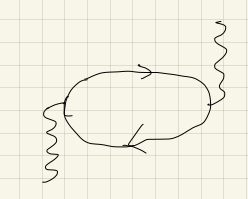
\includegraphics[width=0.2\linewidth]{fig/fig5-9.png}
    \caption{Single--fermion closed loop.}%
    \label{fig:5.9}
\end{figure}
The wiggly lines at each end are just added to define the two vertices of the polarization diagram.
They could indicate that the polarization term is in response to an excitation with wave vector $\bq$ and frequency $i\omega_n$.
The calculation for $\varepsilon_{RPA}$ is not terminated here, sin the terms so far are $ \frac{1}{\varepsilon} = 1 + v_q \mathbf{P}^{(1)} + \dots $ rather that $\varepsilon_{RPA} = 1 - v_q \mathbf{P}^{(1)}$.
Obviously, more terms are needed to get RPA.

The next term in the S-matrix expansion is
\begin{equation}
    \frac{1}{V} \sum_{\bp\bk\bq'} \sum_{\sigma\sigma'} \int_0^\beta d\tau e^{i\omega_n \tau} \int_0^\beta d\tau_1 v_{q'} \langle T_\tau \hat{\rho}(\bq,\tau) \hat{C}^\dagger_{\bp+\bq',\sigma}(\tau_1) \hat{C}^\dagger_{\bk-\bq',\sigma'}(\tau_1) \hat{C}_{\bk\sigma'}(\tau_1) \hat{C}_{\bp\sigma}(\tau_1) \hat{\rho}(-\bq,0) \rangle   \label{5.158}
\end{equation}
There are four terms which result when Wick's theorem is applied to this correlation function.
All contributions have four electron Green's functions and one Coulomb interaction $v_{q'}$. Their diagrms are shown in Figure~\ref{fig:5.10}.
The first one is a vertex correction to the basic bubble diagram.
The next two are exchange energy diagrams for the Green's functions in the bubble;
they contribute the self--energy of these Green's functions.
The last diagram contains two bubbles which are connected by the Coulomb line $v_q$.
\begin{figure}[ht]
    \centering
    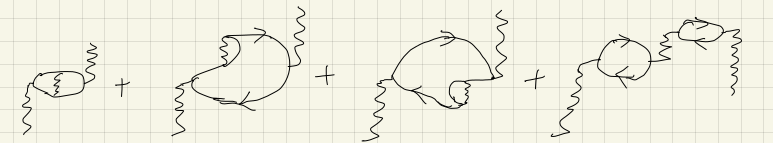
\includegraphics[width=0.8\linewidth]{fig/fig5-10.png}
    \caption{Higher order}%
    \label{fig:5.10}
\end{figure}

Earlier it was remarked that the density--denisty correlation function had the appearance of a Green's function.
It also has a Dyson equation.
The exact evaluation of the correlation functino may be written as\footnote{This is a guess as based on the general form of Green's function.}
\begin{equation}
    - \frac{1}{V} \int_0^\beta d \tau e^{i\omega_n \tau} \langle T_\tau \rho(\bq,\tau) \rho(-\bq,0) \rangle = \frac{\mathbf{P}(\bq,i\omega)}{1 - v_q \mathbf{P}(\bq,\omega)}   \label{5.159}
\end{equation}
There the density operators have the $\tau$ dependence governed by $H=H_0 + V$, instead of only $H_0$ as in $\mathbf{P^{(1)}}$.
The polarization diagram $\mathbf{P}(\bq,i\omega_n)$ is the summation of all \textbf{different} polarization terms.
Polarization diagrams are not "different" if any of their parts are linked by a single Coulomb line $v_q$.
For example teh last diagrme in Figure~\ref{fig:5.10} is not a different polarization diagram.
This term arises from the expansion of geometric series
\begin{equation}
    \frac{P^{(1)}+P^{(2)} + \dots}{1 - v_q \left(P^{(1)} + \dots \right)} = \left( P^{(1)} + \dots \right) \left[ 1 + v_q \left( P^{(1)} + \dots \right) + \dots \right] = P^{(1)} + v_q \left( P^{(1)} \right)^2  + \dots \label{5.160}
\end{equation}
where it is the term $v_q\left( P^{(1)}\right)^2$.
There are terms in $\mathbf{P}(\bq,i\omega_n)$ which have more than one bubble, but they must be connected by more than one Coulomb line.

The random phase approximation is approximating the exact polarization diagram $\mathbf{P}(\bq,i\omega)$ by its first term, which is $\mathbf{P^{(1)}}(\bq,i\omega)$.
The RPA is found from the summation of all single bubble polarization diagrams
\begin{equation}
    \frac{1}{\varepsilon_{RPA}} = 1 + \frac{v_q P^{(1)}}{1 - v_q P^{(1)}} = \frac{1}{1 - v_q P^{(1)}}   \label{5.161}
\end{equation}
which does give $\varepsilon_{RPA} = 1 - v_q P^{(1)}(\bq,i\omega)$.
The eact dielectric function is easily shown to be
\begin{equation}
    \varepsilon(\bq,i\omega) = 1 - v_q \mathbf{P}(\bq,i\omega)  \label{5.162}
\end{equation}
Obviously, to improve the directiic function is to include more terms in the summation of polarization contribution but it is very hard.
In fact, most progress has been made by nondiagramic means, as discussed below.

Using the analytical continuation, the retarded dielectric function is complex
\begin{equation}
    \varepsilon_{RPA} = \varepsilon_1(\bq,\omega) + i \varepsilon_2(\bq,\omega)    \label{5.163}
\end{equation}

The real part $\varepsilon_1$ always approach $1$ at large $\omega$.
At $\omega \to 0$ then $\omega_2 \to 0$, and the static $\varepsilon_{RPA}$ is just $\varepsilon(\bq,0)$.
Using the notation $x=q/2k_F$,
\begin{equation}
    \varepsilon(\bq,0) = 1 + \frac{q^2_{TF}}{2q^2} \left[ 1 + \frac{1}{2x} \left( 1 - x^2 \right) \ln \abs{ \frac{1+x}{1-x} } \right]   \label{5.166}
\end{equation}
which is always positive.
For values $q<k_F$, then $\varepsilon_1(q,\omega)$ becomes negative for intermediate values of $\omega$.
This requres two crossings of the $\varepsilon_1 = 0 $ axis.
The low--frequency crossing always happens when $\varepsilon_2$ is large, so that $-\Im (1/\varepsilon) = \varepsilon_2 / (\varepsilon_1^2 + \varepsilon_2^2 )$ is well behaved when $\varepsilon \approx 0$.
However, the high-frequency point where $\varepsilon_1=0$ has $\varepsilon_2=0$, in that case $ - \Im(1/varepsilon) = \pi \delta(\varepsilon_1)$, so that a delta function is obtained.
This delta function is the plasmon peak which is the sharp singularity on the right of the graph.
Remember that peaks in $S(q,\omega)$ are interpreted as excitations of the system
\begin{equation}
    S(\bq,\omega) = - \frac{1}{n_0 v_q} \Im \left[ \frac{1}{\varepsilon(\bq,\omega)} \right] = \frac{1}{n_0 v_q} \frac{\varepsilon_2}{\varepsilon_1^2 + \varepsilon_2^2}    \label{5.167}
\end{equation}
Plasmons are excitations which exist in real metals and in any electron gas with frequency $\omega^2_0 = \frac{4\pi e^2 n_0}{m}$.

The disscussion abuot the dielectric function is not included in this manuscript.

\subsection{Hubbard}
